% fleqn aligns equations to the left, a4 paper size, 11pt font, article class
\documentclass[fleqn,a4paper,11pt]{article}
\title{Polygonal Cannonball Numbers}
\author{Izaak van Dongen}

\usepackage{mystyle}

\begin{document}
\maketitle\thispagestyle{empty} % no page number under title
\tableofcontents

\section{Introduction}

Recently I watched the video \url{https://www.youtube.com/watch?v=q6L06pyt9CA},
featuring Matt Parker.  Being a huge fan of Matt and of Numperphile, and being
rather full of myself, my first response was naturally one of doubt (also
because of the spirit of mathematical enquiry and all that). I decided to have
my own crack at the problem.

I reasoned that checking if a number is polygonal should be a roughly
\(\BigO(1)\) operation as we can find the \(n\)th term of the base-\(s\)
polygonal numbers \(P(s, n)\), which will be quadratic in \(n\), and solve it
for \(n\) with the quadratic formula, so to check if some cannonball numbers
\(C(s, n_c)\) is polygonal we just see if the corresponding \(n_p\) is an
integer. Now \(10^9\) is a fairly small number. Seeing as my CPU's clockspeed is
in the range of gigahertz, and we're just checking a tiny fraction of those
numbers as we're just computing the cannonball numbers under this limit, it
seems reasonable that this should be doable fairly fast.

I've thought about the problem of higher-dimensional stacks of cannonballs (ie
the ones formed by adding up the cannonball numbers), but I've not done anything
about it.

\section{The Maths}

Indeed, this approach does seem to work. Almost by definition we have the
recurrence in polygonal numbers
\begin{equation*}
P(s, n) = P(s, n - 1) + n(s - 2) - (s - 3)
\end{equation*}
so we can use
\begin{align*}
P(s, n) &= \sum_{r = 1}^n P(s, r) - P(s, r - 1) \\
    &= \sum_{r = 1}^n (n(s - 2) - (s - 3)) \\
    &= \frac 12 n(n + 1)(s - 2) - n(s - 3) \\
    &= \frac{n^2(s - 2) - n(s - 4)} 2
\end{align*}
Fortunately this seems to agree with what Wikipedia thinks. Now, we have
\begin{alignat*}{2}
&& 0 &= (s - 2)n^2 - (s - 4)n - 2P(s, n) \\
&\implies& n &= \frac{s - 4 + \sqrt{(s - 4)^2 + 8(s - 2)P(s, n)}}{2s - 4}
\end{alignat*}
Wikipedia still seems to think we're on track.

Another result that I don't really use is that
\begin{align*}
C(s, n) &= \sum_{r = 1}^n P(s, n) \\
    &= \frac 12 \sum_{r = 1}^n (n^2(s - 2) - n(s - 4)) \\
    &= \frac 12 \pqty{\frac{n(n + 1)(2n + 1)(s - 2)} 6
                    - \frac{n(n + 1)(s - 4)} 2} \\
    &= \frac 1{12}n(n + 1)\bqty{(2n + 1)(s - 2) - 3(s - 4)}
\end{align*}
In fact I've only used this in verification of the results.

Regardless, now we need only work our way up the \(C(s, n)\)s using the
recurrence \(C(s, n) = P(s, n) + C(s, n - 1)\), and check for each if the
quadratic formula gives an integer result. This is most easily done by checking
if the discriminant is a perfect square and then checking that the denominator
divides the numerator.

\section{The Programming}

For speeeeeeed I implemented this in C (although there is a long abandoned
parallel Python implementation). I used 128-bit integers to be on the safe side,
as \(10^{19}\) is a little small for my liking. This meant I had to do a lot of
messing around to get things to actually display in base 10.

I did briefly consider either implementing or importing some kind of arbitrary
precision integer arithmetic functionality, but then I decided I wasn't going to
run it on anything fast enough to have to worry about that, and I have better
things to do.

There's also a slick little progress update that gets printed to STDERR, and a
number of zsh scripts to save me typing.

\section{The Ugly}

Table \ref{tab_ugly} lists all the solutions that I've found, so far. The \TeX
source of the table is in \texttt{../src/tab.tex}, which is derived from
\texttt{../src/c/solutions/*}.

I have also plotted both the data in its entirety on a double logarithmic scale
\ref{fig_lin}, and an excerpt from the data on a linear scale (\ref{fig_log}).

The obvious pattern that jumps out is the big line of points for all the sides
congrent to \(2 \pmod 3\). Particularly because it looks like such a straight
line on the log-log plot, we would expect it to be modelled well as a constant
multiple of some power of \(s\). I drew two lines that seemed to roughly bound
it, and used those to extract the points on the line and then do some linear
regression on that (figure \ref{fig_log_interesting}. I obtained the formula
\begin{equation*}
C = 0.003828399 \cdot s ^ { 7.068495 }
\end{equation*}
which seems to be accurate to within probably about \(1\%\), I've not really
checked properly.

\begin{figure}[H]
\centering
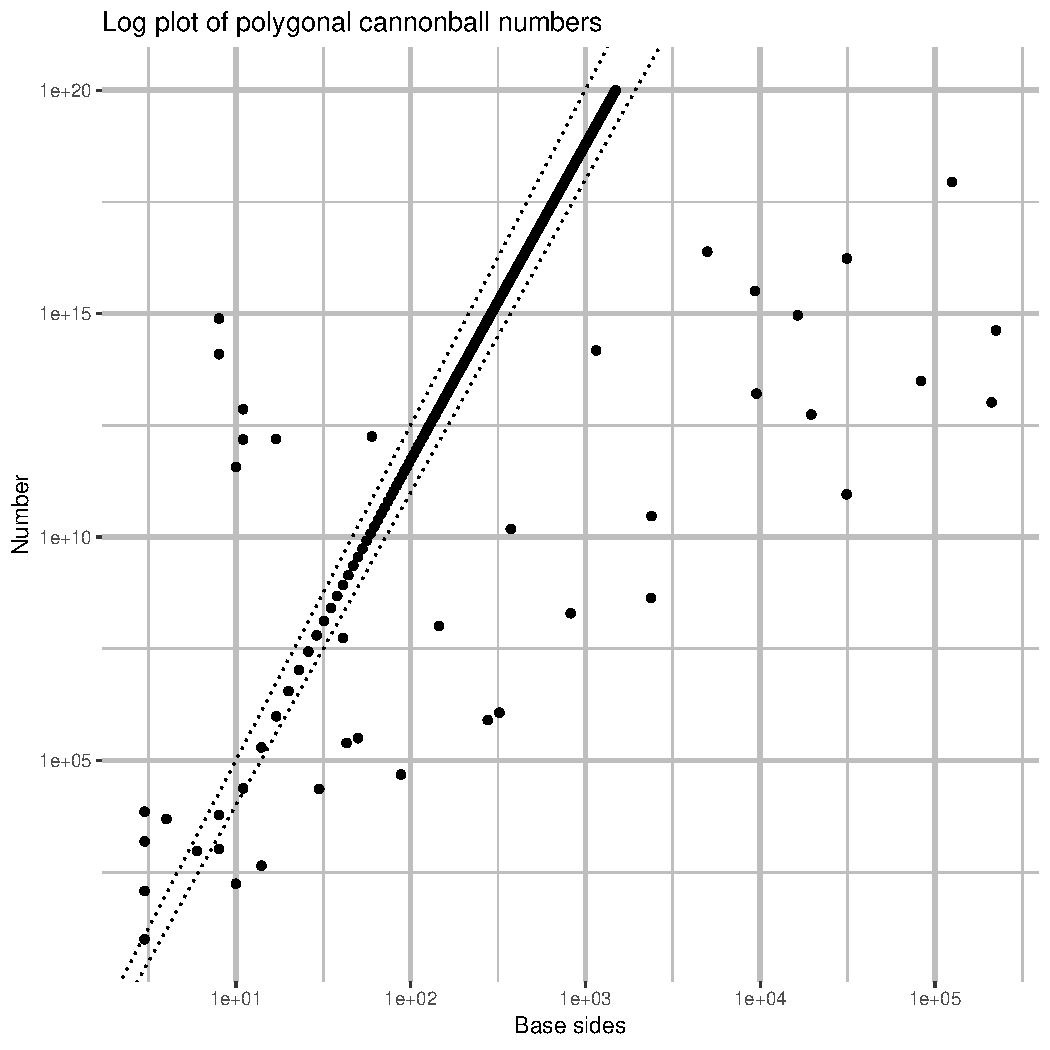
\includegraphics[width=\textwidth,page=1]{../graph/Rplots.pdf}
\caption{Log plot}
\label{fig_log}
\end{figure}

\begin{figure}[H]
\centering
\includegraphics[width=\textwidth,page=2]{../graph/Rplots.pdf}
\caption{Linear plot}
\label{fig_lin}
\end{figure}

\begin{figure}[H]
\centering
\includegraphics[width=\textwidth,page=3]{../graph/Rplots.pdf}
\caption{Log plot of the interesting bit}
\label{fig_log_interesting}
\end{figure}

\begin{longtable}{*4r}
\toprule
\boldmath \(s\) & \boldmath \(C(s, n_c) = P(s, n_p)\)
& \boldmath \(n_p\) & \boldmath \(n_c\) \\
\midrule
\endhead
3 & 10 & 4 & 3 \\
3 & 120 & 15 & 8 \\
3 & 1540 & 55 & 20 \\
3 & 7140 & 119 & 34 \\
4 & 4900 & 70 & 24 \\
6 & 946 & 22 & 11 \\
8 & 1045 & 19 & 10 \\
8 & 5985 & 45 & 18 \\
8 & 123395663059845 & 6413415 & 49785 \\
8 & 774611255177760 & 16068720 & 91839 \\
10 & 175 & 7 & 5 \\
10 & 368050005576 & 303336 & 6511 \\
11 & 23725 & 73 & 25 \\
11 & 1519937678700 & 581175 & 10044 \\
11 & 7248070597636 & 1269127 & 16906 \\
14 & 441 & 9 & 6 \\
14 & 195661 & 181 & 46 \\
17 & 975061 & 361 & 73 \\
17 & 1580765544996 & 459096 & 8583 \\
20 & 3578401 & 631 & 106 \\
23 & 10680265 & 1009 & 145 \\
26 & 27453385 & 1513 & 190 \\
29 & 63016921 & 2161 & 241 \\
30 & 23001 & 41 & 17 \\
32 & 132361021 & 2971 & 298 \\
35 & 258815701 & 3961 & 361 \\
38 & 477132085 & 5149 & 430 \\
41 & 55202400 & 1683 & 204 \\
41 & 837244045 & 6553 & 505 \\
43 & 245905 & 110 & 33 \\
44 & 1408778281 & 8191 & 586 \\
47 & 2286380881 & 10081 & 673 \\
50 & 314755 & 115 & 34 \\
50 & 3595928401 & 12241 & 766 \\
53 & 5501691505 & 14689 & 865 \\
56 & 8214519205 & 17443 & 970 \\
59 & 12001111741 & 20521 & 1081 \\
60 & 1785508245600 & 248132 & 5695 \\
62 & 17194450141 & 23941 & 1198 \\
65 & 24205450501 & 27721 & 1321 \\
68 & 33535911025 & 31879 & 1450 \\
71 & 45792819865 & 36433 & 1585 \\
74 & 61704091801 & 41401 & 1726 \\
77 & 82135801801 & 46801 & 1873 \\
80 & 108110983501 & 52651 & 2026 \\
83 & 140830060645 & 58969 & 2185 \\
86 & 181692979525 & 65773 & 2350 \\
88 & 48280 & 34 & 15 \\
89 & 232323110461 & 73081 & 2521 \\
92 & 294592986361 & 80911 & 2698 \\
95 & 370651946401 & 89281 & 2881 \\
98 & 462955752865 & 98209 & 3070 \\
101 & 574298249185 & 107713 & 3265 \\
104 & 707845127221 & 117811 & 3466 \\
107 & 867169871821 & 128521 & 3673 \\
110 & 1056291950701 & 139861 & 3886 \\
113 & 1279717317685 & 151849 & 4105 \\
116 & 1542481297345 & 164503 & 4330 \\
119 & 1850193919081 & 177841 & 4561 \\
122 & 2209087768681 & 191881 & 4798 \\
125 & 2626068425401 & 206641 & 5041 \\
128 & 3108767552605 & 222139 & 5290 \\
131 & 3665598710005 & 238393 & 5545 \\
134 & 4305815955541 & 255421 & 5806 \\
137 & 5039575304941 & 273241 & 6073 \\
140 & 5877999117001 & 291871 & 6346 \\
143 & 6833243472625 & 311329 & 6625 \\
145 & 101337426 & 1191 & 162 \\
146 & 7918568615665 & 331633 & 6910 \\
149 & 9148412523601 & 352801 & 7201 \\
152 & 10538467676101 & 374851 & 7498 \\
155 & 12105761089501 & 397801 & 7801 \\
158 & 13868737685245 & 421669 & 8110 \\
161 & 15847347060325 & 446473 & 8425 \\
164 & 18063133727761 & 472231 & 8746 \\
167 & 20539330895161 & 498961 & 9073 \\
170 & 23300957849401 & 526681 & 9406 \\
173 & 26374921015465 & 555409 & 9745 \\
176 & 29790118757485 & 585163 & 10090 \\
179 & 33577549990021 & 615961 & 10441 \\
182 & 37770426667621 & 647821 & 10798 \\
185 & 42404290220701 & 680761 & 11161 \\
188 & 47517132005785 & 714799 & 11530 \\
191 & 53149517838145 & 749953 & 11905 \\
194 & 59344716674881 & 786241 & 12286 \\
197 & 66148833516481 & 823681 & 12673 \\
200 & 73610946594901 & 862291 & 13066 \\
203 & 81783248916205 & 902089 & 13465 \\
206 & 90721194225805 & 943093 & 13870 \\
209 & 100483647464341 & 985321 & 14281 \\
212 & 111133039782241 & 1028791 & 14698 \\
215 & 122735528181001 & 1073521 & 15121 \\
218 & 135361159849225 & 1119529 & 15550 \\
221 & 149084041261465 & 1166833 & 15985 \\
224 & 163982512107901 & 1215451 & 16426 \\
227 & 180139324122901 & 1265401 & 16873 \\
230 & 197641824880501 & 1316701 & 17326 \\
233 & 216582146624845 & 1369369 & 17785 \\
236 & 237057400203625 & 1423423 & 18250 \\
239 & 259169874172561 & 1478881 & 18721 \\
242 & 283027239138961 & 1535761 & 19198 \\
245 & 308742757412401 & 1594081 & 19681 \\
248 & 336435498030565 & 1653859 & 20170 \\
251 & 366230557228285 & 1715113 & 20665 \\
254 & 398259284417821 & 1777861 & 21166 \\
257 & 432659513748421 & 1842121 & 21673 \\
260 & 469575801313201 & 1907911 & 22186 \\
263 & 509159668071385 & 1975249 & 22705 \\
266 & 551569848553945 & 2044153 & 23230 \\
269 & 596972545420681 & 2114641 & 23761 \\
272 & 645541689936781 & 2186731 & 24298 \\
275 & 697459208436901 & 2260441 & 24841 \\
276 & 801801 & 77 & 26 \\
278 & 752915294844805 & 2335789 & 25390 \\
281 & 812108689316605 & 2412793 & 25945 \\
284 & 875246963075641 & 2491471 & 26506 \\
287 & 942546809507041 & 2571841 & 27073 \\
290 & 1014234341580001 & 2653921 & 27646 \\
293 & 1090545395665825 & 2737729 & 28225 \\
296 & 1171725841819765 & 2823283 & 28810 \\
299 & 1258031900594701 & 2910601 & 29401 \\
302 & 1349730466454701 & 2999701 & 29998 \\
305 & 1447099437856501 & 3090601 & 30601 \\
308 & 1550428054066945 & 3183319 & 31210 \\
311 & 1660017238784425 & 3277873 & 31825 \\
314 & 1776179950632361 & 3374281 & 32446 \\
317 & 1899241540592761 & 3472561 & 33073 \\
320 & 2029540116447901 & 3572731 & 33706 \\
322 & 1169686 & 86 & 28 \\
323 & 2167426914298165 & 3674809 & 34345 \\
326 & 2313266677224085 & 3778813 & 34990 \\
329 & 2467438041160621 & 3884761 & 35641 \\
332 & 2630333928051721 & 3992671 & 36298 \\
335 & 2802361946353201 & 4102561 & 36961 \\
338 & 2983944798951985 & 4214449 & 37630 \\
341 & 3175520698569745 & 4328353 & 38305 \\
344 & 3377543790718981 & 4444291 & 38986 \\
347 & 3590484584279581 & 4562281 & 39673 \\
350 & 3814830389763901 & 4682341 & 40366 \\
353 & 4051085765338405 & 4804489 & 41065 \\
356 & 4299772970669905 & 4928743 & 41770 \\
359 & 4561432428664441 & 5055121 & 42481 \\
362 & 4836623195166841 & 5183641 & 43198 \\
365 & 5125923436689001 & 5314321 & 43921 \\
368 & 5429930916234925 & 5447179 & 44650 \\
371 & 5749263487290565 & 5582233 & 45385 \\
374 & 15064335000 & 9000 & 624 \\
374 & 6084559596046501 & 5719501 & 46126 \\
377 & 6436478791921501 & 5859001 & 46873 \\
380 & 6805702246455001 & 6000751 & 47626 \\
383 & 7192933280636545 & 6144769 & 48385 \\
386 & 7598897900740225 & 6291073 & 49150 \\
389 & 8024345342732161 & 6439681 & 49921 \\
392 & 8470048625319061 & 6590611 & 50698 \\
395 & 8936805111705901 & 6743881 & 51481 \\
398 & 9425437080130765 & 6899509 & 52270 \\
401 & 9936792303244885 & 7057513 & 53065 \\
404 & 10471744636405921 & 7217911 & 53866 \\
407 & 11031194614952521 & 7380721 & 54673 \\
410 & 11616070060528201 & 7545961 & 55486 \\
413 & 12227326696522585 & 7713649 & 56305 \\
416 & 12865948772698045 & 7883803 & 57130 \\
419 & 13532949699069781 & 8056441 & 57961 \\
422 & 14229372689107381 & 8231581 & 58798 \\
425 & 14956291412325901 & 8409241 & 59641 \\
428 & 15714810656334505 & 8589439 & 60490 \\
431 & 16506066998410705 & 8772193 & 61345 \\
434 & 17331229486668241 & 8957521 & 62206 \\
437 & 18191500330886641 & 9145441 & 63073 \\
440 & 19088115603070501 & 9335971 & 63946 \\
443 & 20022345947806525 & 9529129 & 64825 \\
446 & 20995497302486365 & 9724933 & 65710 \\
449 & 22008911627463301 & 9923401 & 66601 \\
452 & 23063967646210801 & 10124551 & 67498 \\
455 & 24162081595551001 & 10328401 & 68401 \\
458 & 25304707986021145 & 10534969 & 69310 \\
461 & 26493340372446025 & 10744273 & 70225 \\
464 & 27729512134784461 & 10956331 & 71146 \\
467 & 29014797269317861 & 11171161 & 72073 \\
470 & 30350811190248901 & 11388781 & 73006 \\
473 & 31739211541778365 & 11609209 & 73945 \\
476 & 33181699020728185 & 11832463 & 74890 \\
479 & 34680018209778721 & 12058561 & 75841 \\
482 & 36235958421388321 & 12287521 & 76798 \\
485 & 37851354552463201 & 12519361 & 77761 \\
488 & 39528087949845685 & 12754099 & 78730 \\
491 & 41268087286688845 & 12991753 & 79705 \\
494 & 43073329449785581 & 13232341 & 80686 \\
497 & 44945840437920181 & 13475881 & 81673 \\
500 & 46887696271310401 & 13722391 & 82666 \\
503 & 48901023912208105 & 13971889 & 83665 \\
506 & 50988002196726505 & 14224393 & 84670 \\
509 & 53150862777962041 & 14479921 & 85681 \\
512 & 55391891080478941 & 14738491 & 86698 \\
515 & 57713427266224501 & 15000121 & 87721 \\
518 & 60117867211943125 & 15264829 & 88750 \\
521 & 62607663498157165 & 15532633 & 89785 \\
524 & 65185326409782601 & 15803551 & 90826 \\
527 & 67853424948447601 & 16077601 & 91873 \\
530 & 70614587856582001 & 16354801 & 92926 \\
533 & 73471504653345745 & 16635169 & 93985 \\
536 & 76426926682464325 & 16918723 & 95050 \\
539 & 79483668172039261 & 17205481 & 96121 \\
542 & 82644607306401661 & 17495461 & 97198 \\
545 & 85912687310076901 & 17788681 & 98281 \\
548 & 89290917543928465 & 18085159 & 99370 \\
551 & 92782374613548985 & 18384913 & 100465 \\
554 & 96390203489966521 & 18687961 & 101566 \\
557 & 100117618642734121 & 18994321 & 102673 \\
560 & 103967905185470701 & 19304011 & 103786 \\
563 & 107944420033921285 & 19617049 & 104905 \\
566 & 112050593076604645 & 19933453 & 106030 \\
569 & 116289928358116381 & 20253241 & 107161 \\
572 & 120666005275155481 & 20576431 & 108298 \\
575 & 125182479785342401 & 20903041 & 109441 \\
578 & 129843085628896705 & 21233089 & 110590 \\
581 & 134651635563242305 & 21566593 & 111745 \\
584 & 139612022610608341 & 21903571 & 112906 \\
587 & 144728221318693741 & 22244041 & 114073 \\
590 & 150004289034463501 & 22588021 & 115246 \\
593 & 155444367191144725 & 22935529 & 116425 \\
596 & 161052682608490465 & 23286583 & 117610 \\
599 & 166833548806379401 & 23641201 & 118801 \\
602 & 172791367331819401 & 23999401 & 119998 \\
605 & 178930629099423001 & 24361201 & 121201 \\
608 & 185255915745422845 & 24726619 & 122410 \\
611 & 191771900995295125 & 25095673 & 123625 \\
614 & 198483352045059061 & 25468381 & 124846 \\
617 & 205395130956320461 & 25844761 & 126073 \\
620 & 212512196065127401 & 26224831 & 127306 \\
623 & 219839603404706065 & 26608609 & 128545 \\
626 & 227382508142144785 & 26996113 & 129790 \\
629 & 235146166029094321 & 27387361 & 131041 \\
632 & 243135934866552421 & 27782371 & 132298 \\
635 & 251357275983800701 & 28181161 & 133561 \\
638 & 259815755731561885 & 28583749 & 134830 \\
641 & 268517046989445445 & 28990153 & 136105 \\
644 & 277466930687749681 & 29400391 & 137386 \\
647 & 286671297343688281 & 29814481 & 138673 \\
650 & 296136148612109401 & 30232441 & 139966 \\
653 & 305867598850775305 & 30654289 & 141265 \\
656 & 315871876700270605 & 31080043 & 142570 \\
659 & 326155326678607141 & 31509721 & 143881 \\
662 & 336724410790593541 & 31943341 & 145198 \\
665 & 347585710152037501 & 32380921 & 146521 \\
668 & 358745926628848825 & 32822479 & 147850 \\
671 & 370211884491111265 & 33268033 & 149185 \\
674 & 381990532082191201 & 33717601 & 150526 \\
677 & 394088943502951201 & 34171201 & 151873 \\
680 & 406514320311136501 & 34628851 & 153226 \\
683 & 419273993236002445 & 35090569 & 154585 \\
686 & 432375423908250925 & 35556373 & 155950 \\
689 & 445826206605343861 & 36026281 & 157321 \\
692 & 459634070012261761 & 36500311 & 158698 \\
695 & 473806878997775401 & 36978481 & 160081 \\
698 & 488352636406298665 & 37460809 & 161470 \\
701 & 503279484865390585 & 37947313 & 162865 \\
704 & 518595708608974621 & 38438011 & 164266 \\
707 & 534309735316343221 & 38932921 & 165673 \\
710 & 550430137967015701 & 39432061 & 167086 \\
713 & 566965636711517485 & 39935449 & 168505 \\
716 & 583925100758148745 & 40443103 & 169930 \\
719 & 601317550275810481 & 40955041 & 171361 \\
722 & 619152158312956081 & 41471281 & 172798 \\
725 & 637438252732736401 & 41991841 & 174241 \\
728 & 656185318164406405 & 42516739 & 175690 \\
731 & 675402997971061405 & 43045993 & 177145 \\
734 & 695101096233770941 & 43579621 & 178606 \\
737 & 715289579752178341 & 44117641 & 180073 \\
740 & 735978580061634001 & 44660071 & 181546 \\
743 & 757178395466930425 & 45206929 & 183025 \\
746 & 778899493092707065 & 45758233 & 184510 \\
749 & 801152510950593001 & 46314001 & 186001 \\
752 & 823948260023155501 & 46874251 & 187498 \\
755 & 847297726364722501 & 47439001 & 189001 \\
758 & 871212073219147045 & 48008269 & 190510 \\
761 & 895702643154581725 & 48582073 & 192025 \\
764 & 920780960215331161 & 49160431 & 193546 \\
767 & 946458732090850561 & 49743361 & 195073 \\
770 & 972747852301958401 & 50330881 & 196606 \\
773 & 999660402404331265 & 50923009 & 198145 \\
776 & 1027208654209348885 & 51519763 & 199690 \\
779 & 1055405072022357421 & 52121161 & 201241 \\
782 & 1084262314898419021 & 52727221 & 202798 \\
785 & 1113793238915615701 & 53337961 & 204361 \\
788 & 1144010899465975585 & 53953399 & 205930 \\
791 & 1174928553564089545 & 54573553 & 207505 \\
794 & 1206559662173486281 & 55198441 & 209086 \\
797 & 1238917892550833881 & 55828081 & 210673 \\
800 & 1272017120608035901 & 56462491 & 212266 \\
803 & 1305871433292290005 & 57101689 & 213865 \\
806 & 1340495130984177205 & 57745693 & 215470 \\
809 & 1375902729913849741 & 58394521 & 217081 \\
812 & 1412108964595385641 & 59048191 & 218698 \\
815 & 1449128790279378001 & 59706721 & 220321 \\
818 & 1486977385423827025 & 60370129 & 221950 \\
821 & 1525670154183402865 & 61038433 & 223585 \\
823 & 197427385 & 694 & 113 \\
824 & 1565222728917147301 & 61711651 & 225226 \\
827 & 1605650972714682301 & 62389801 & 226873 \\
830 & 1646970981940993501 & 63072901 & 228526 \\
833 & 1689199088799856645 & 63760969 & 230185 \\
836 & 1732351863915975025 & 64454023 & 231850 \\
839 & 1776446118935895961 & 65152081 & 233521 \\
842 & 1821498909147774361 & 65855161 & 235198 \\
845 & 1867527536120051401 & 66563281 & 236881 \\
848 & 1914549550359116365 & 67276459 & 238570 \\
851 & 1962582753986019685 & 67994713 & 240265 \\
854 & 2011645203432305221 & 68718061 & 241966 \\
857 & 2061755212155029821 & 69446521 & 243673 \\
860 & 2112931353371038201 & 70180111 & 245386 \\
863 & 2165192462810561185 & 70918849 & 247105 \\
866 & 2218557641490205345 & 71662753 & 248830 \\
869 & 2273046258505402081 & 72411841 & 250561 \\
872 & 2328677953842384181 & 73166131 & 252298 \\
875 & 2385472641209757901 & 73925641 & 254041 \\
878 & 2443450510889738605 & 74690389 & 255790 \\
881 & 2502632032609118005 & 75460393 & 257545 \\
884 & 2563037958430031041 & 76235671 & 259306 \\
887 & 2624689325660590441 & 77016241 & 261073 \\
890 & 2687607459785457001 & 77802121 & 262846 \\
893 & 2751813977416413625 & 78593329 & 264625 \\
896 & 2817330789263011165 & 79389883 & 266410 \\
899 & 2884180103123354101 & 80191801 & 268201 \\
902 & 2952384426895094101 & 80999101 & 269998 \\
905 & 3021966571606699501 & 81811801 & 271801 \\
908 & 3092949654469068745 & 82629919 & 273610 \\
911 & 3165357101947555825 & 83453473 & 275425 \\
914 & 3239212652854475761 & 84282481 & 277246 \\
917 & 3314540361462158161 & 85116961 & 279073 \\
920 & 3391364600636616901 & 85956931 & 280906 \\
923 & 3469710064991903965 & 86802409 & 282745 \\
926 & 3549601774065215485 & 87653413 & 284590 \\
929 & 3631065075512818021 & 88509961 & 286441 \\
932 & 3714125648326863121 & 89372071 & 288298 \\
935 & 3798809506073158201 & 90239761 & 290161 \\
938 & 3885143000149961785 & 91113049 & 292030 \\
941 & 3973152823067871145 & 91991953 & 293905 \\
944 & 4062866011750870381 & 92876491 & 295786 \\
947 & 4154309950858606981 & 93766681 & 297673 \\
950 & 4247512376129964901 & 94662541 & 299566 \\
953 & 4342501377748002205 & 95564089 & 301465 \\
956 & 4439305403726321305 & 96471343 & 303370 \\
959 & 4537953263316939841 & 97384321 & 305281 \\
962 & 4638474130439730241 & 98303041 & 307198 \\
965 & 4740897547133496001 & 99227521 & 309121 \\
968 & 4845253427028752725 & 100157779 & 311050 \\
971 & 4951572058842281965 & 101093833 & 312985 \\
974 & 5059884109893525901 & 102035701 & 314926 \\
977 & 5170220629642890901 & 102983401 & 316873 \\
980 & 5282613053252028001 & 103936951 & 318826 \\
983 & 5397093205166158345 & 104896369 & 320785 \\
986 & 5513693302718511625 & 105861673 & 322750 \\
989 & 5632445959756945561 & 106832881 & 324721 \\
992 & 5753384190292814461 & 107810011 & 326698 \\
995 & 5876541412172154901 & 108793081 & 328681 \\
998 & 6001951450769256565 & 109782109 & 330670 \\
1001 & 6129648542702686285 & 110777113 & 332665 \\
1004 & 6259667339573833321 & 111778111 & 334666 \\
1007 & 6392042911728043921 & 112785121 & 336673 \\
1010 & 6526810752038413201 & 113798161 & 338686 \\
1013 & 6664006779712302385 & 114817249 & 340705 \\
1016 & 6803667344120649445 & 115842403 & 342730 \\
1019 & 6945829228650141181 & 116873641 & 344761 \\
1022 & 7090529654578314781 & 117910981 & 346798 \\
1025 & 7237806284971656901 & 118954441 & 348841 \\
1028 & 7387697228606768305 & 120004039 & 350890 \\
1031 & 7540241043914662105 & 121059793 & 352945 \\
1034 & 7695476742948263641 & 122121721 & 355006 \\
1037 & 7853443795373180041 & 123189841 & 357073 \\
1040 & 8014182132481807501 & 124264171 & 359146 \\
1043 & 8177732151230844325 & 125344729 & 361225 \\
1046 & 8344134718302277765 & 126431533 & 363310 \\
1049 & 8513431174187912701 & 127524601 & 365401 \\
1052 & 8685663337297510201 & 128623951 & 367498 \\
1055 & 8860873508090604001 & 129729601 & 369601 \\
1058 & 9039104473232062945 & 130841569 & 371710 \\
1061 & 9220399509771467425 & 131959873 & 373825 \\
1064 & 9404802389346367861 & 133084531 & 375946 \\
1067 & 9592357382409493261 & 134215561 & 378073 \\
1070 & 9783109262479977901 & 135352981 & 380206 \\
1073 & 9977103310418674165 & 136496809 & 382345 \\
1076 & 10174385318727619585 & 137647063 & 384490 \\
1079 & 10375001595873726121 & 138803761 & 386641 \\
1082 & 10578998970636759721 & 139966921 & 388798 \\
1085 & 10786424796481678201 & 141136561 & 390961 \\
1088 & 10997326955955395485 & 142312699 & 393130 \\
1091 & 11211753865108040245 & 143495353 & 395305 \\
1094 & 11429754477938776981 & 144684541 & 397486 \\
1097 & 11651378290866257581 & 145880281 & 399673 \\
1100 & 11876675347223771401 & 147082591 & 401866 \\
1103 & 12105696241779161905 & 148291489 & 404065 \\
1106 & 12338492125279577905 & 149506993 & 406270 \\
1109 & 12575114709021127441 & 150729121 & 408481 \\
1112 & 12815616269443502341 & 151957891 & 410698 \\
1115 & 13060049652749641501 & 153193321 & 412921 \\
1118 & 13308468279550500925 & 154435429 & 415150 \\
1121 & 13560926149534998565 & 155684233 & 417385 \\
1124 & 13817477846165202001 & 156939751 & 419626 \\
1127 & 14078178541396827001 & 158202001 & 421873 \\
1130 & 14343084000425115001 & 159471001 & 424126 \\
1133 & 14612250586456157545 & 160746769 & 426385 \\
1136 & 14885735265503735725 & 162029323 & 428650 \\
1139 & 15163595611211742661 & 163318681 & 430921 \\
1142 & 15445889809702257061 & 164614861 & 433198 \\
1145 & 15732676664449335901 & 165917881 & 435481 \\
1148 & 16024015601178594265 & 167227759 & 437770 \\
1151 & 16319966672792640385 & 168544513 & 440065 \\
1152 & 149979784926720 & 510720 & 9215 \\
1154 & 16620590564322433921 & 169868161 & 442366 \\
1157 & 16925948597904635521 & 171198721 & 444673 \\
1160 & 17236102737785015701 & 172536211 & 446986 \\
1163 & 17551115595347991085 & 173880649 & 449305 \\
1166 & 17871050434172356045 & 175232053 & 451630 \\
1169 & 18195971175113277781 & 176590441 & 453961 \\
1172 & 18525942401410622881 & 177955831 & 456298 \\
1175 & 18861029363823683401 & 179328241 & 458641 \\
1178 & 19201297985792370505 & 180707689 & 460990 \\
1181 & 19546814868624943705 & 182094193 & 463345 \\
1184 & 19897647296712343741 & 183487771 & 465706 \\
1187 & 20253863242769197141 & 184888441 & 468073 \\
1190 & 20615531373101560501 & 186296221 & 470446 \\
1193 & 20982721052901472525 & 187711129 & 472825 \\
1196 & 21355502351568381865 & 189133183 & 475210 \\
1199 & 21733946048057518801 & 190562401 & 477601 \\
1202 & 22118123636255278801 & 191998801 & 479998 \\
1205 & 22508107330381686001 & 193442401 & 482401 \\
1208 & 22903970070420004645 & 194893219 & 484810 \\
1211 & 23305785527573566525 & 196351273 & 487225 \\
1214 & 23713628109749882461 & 197816581 & 489646 \\
1217 & 24127572967072105861 & 199289161 & 492073 \\
1220 & 24547695997417916401 & 200769031 & 494506 \\
1223 & 24974073851985891865 & 202256209 & 496945 \\
1226 & 25406783940889436185 & 203750713 & 499390 \\
1229 & 25845904438778331721 & 205252561 & 501841 \\
1232 & 26291514290487983821 & 206761771 & 504298 \\
1235 & 26743693216716425701 & 208278361 & 506761 \\
1238 & 27202521719729151685 & 209802349 & 509230 \\
1241 & 27668081089091846845 & 211333753 & 511705 \\
1244 & 28140453407431081081 & 212872591 & 514186 \\
1247 & 28619721556223035681 & 214418881 & 516673 \\
1250 & 29105969221610330401 & 215972641 & 519166 \\
1253 & 29599280900247019105 & 217533889 & 521665 \\
1256 & 30099741905171822005 & 219102643 & 524170 \\
1259 & 30607438371709662541 & 220678921 & 526681 \\
1262 & 31122457263401576941 & 222262741 & 529198 \\
1265 & 31644886377963064501 & 223854121 & 531721 \\
1268 & 32174814353270946625 & 225453079 & 534250 \\
1271 & 32712330673378802665 & 227059633 & 536785 \\
1274 & 33257525674561050601 & 228673801 & 539326 \\
1277 & 33810490551385740601 & 230295601 & 541873 \\
1280 & 34371317362816129501 & 231925051 & 544426 \\
1283 & 34940099038341104245 & 233562169 & 546985 \\
1286 & 35516929384134522325 & 235206973 & 549550 \\
1289 & 36101903089243537261 & 236859481 & 552121 \\
1292 & 36695115731805977161 & 238519711 & 554698 \\
1295 & 37296663785296844401 & 240187681 & 557281 \\
1298 & 37906644624804004465 & 241863409 & 559870 \\
1301 & 38525156533333131985 & 243546913 & 562465 \\
1304 & 39152298708141982021 & 245238211 & 565066 \\
1307 & 39788171267104054621 & 246937321 & 567673 \\
1310 & 40432875255101720701 & 248644261 & 570286 \\
1313 & 41086512650448877285 & 250359049 & 572905 \\
1316 & 41749186371343200145 & 252081703 & 575530 \\
1319 & 42421000282348061881 & 253812241 & 578161 \\
1322 & 43102059200904183481 & 255550681 & 580798 \\
1325 & 43792468903871087401 & 257297041 & 583441 \\
1328 & 44492336134098420205 & 259051339 & 586090 \\
1331 & 45201768607027212805 & 260813593 & 588745 \\
1334 & 45920875017321146341 & 262583821 & 591406 \\
1337 & 46649765045527891741 & 264362041 & 594073 \\
1340 & 47388549364770591001 & 266148271 & 596746 \\
1343 & 48137339647469548225 & 267942529 & 599425 \\
1346 & 48896248572094198465 & 269744833 & 602110 \\
1349 & 49665389829945422401 & 271555201 & 604801 \\
1352 & 50444878131968274901 & 273373651 & 607498 \\
1355 & 51234829215595195501 & 275200201 & 610201 \\
1358 & 52035359851619768845 & 277034869 & 612910 \\
1361 & 52846587851101103125 & 278877673 & 615625 \\
1364 & 53668632072298894561 & 280728631 & 618346 \\
1367 & 54501612427639245961 & 282587761 & 621073 \\
1370 & 55345649890711307401 & 284455081 & 623806 \\
1373 & 56200866503294807065 & 286330609 & 626545 \\
1376 & 57067385382418540285 & 288214363 & 629290 \\
1379 & 57945330727449884821 & 290106361 & 632041 \\
1382 & 58834827827215410421 & 292006621 & 634798 \\
1385 & 59736003067152650701 & 293915161 & 637561 \\
1388 & 60648983936493105385 & 295831999 & 640330 \\
1391 & 61573899035476540945 & 297757153 & 643105 \\
1394 & 62510878082596657681 & 299690641 & 645886 \\
1397 & 63460051921878191281 & 301632481 & 648673 \\
1400 & 64421552530185516901 & 303582691 & 651466 \\
1403 & 65395513024562823805 & 305541289 & 654265 \\
1406 & 66382067669605928605 & 307508293 & 657070 \\
1409 & 67381351884865795141 & 309483721 & 659881 \\
1412 & 68393502252283829041 & 311467591 & 662698 \\
1415 & 69418656523659015001 & 313459921 & 665521 \\
1418 & 70456953628146964825 & 315460729 & 668350 \\
1421 & 71508533679790944265 & 317470033 & 671185 \\
1424 & 72573537985084946701 & 319487851 & 674026 \\
1427 & 73652109050568881701 & 321514201 & 676873 \\
1430 & 74744390590455946501 & 323549101 & 679726 \\
1433 & 75850527534292248445 & 325592569 & 682585 \\
1436 & 76970666034648746425 & 327644623 & 685450 \\
1439 & 78104953474845579361 & 329705281 & 688321 \\
1442 & 79253538476708849761 & 331774561 & 691198 \\
1445 & 80416570908359930401 & 333852481 & 694081 \\
1448 & 81594201892037362165 & 335939059 & 696970 \\
1451 & 82786583811951411085 & 338034313 & 699865 \\
1454 & 83993870322171352621 & 340138261 & 702766 \\
1457 & 85216216354545551221 & 342250921 & 705673 \\
1460 & 86453778126654403201 & 344372311 & 708586 \\
1463 & 87706713149796210985 & 346502449 & 711505 \\
1466 & 88975180237006056745 & 348641353 & 714430 \\
1469 & 90259339511107743481 & 350789041 & 717361 \\
1472 & 91559352412798871581 & 352945531 & 720298 \\
1475 & 92875381708769118901 & 355110841 & 723241 \\
1478 & 94207591499851792405 & 357284989 & 726190 \\
1481 & 95556147229208719405 & 359467993 & 729145 \\
1484 & 96921215690548546441 & 361659871 & 732106 \\
1487 & 98302965036378513841 & 363860641 & 735073 \\
1490 & 99701564786289774001 & 366070321 & 738046 \\
2378 & 432684460 & 604 & 103 \\
2386 & 29437553530 & 4970 & 420 \\
4980 & 24264913354964425 & 3122317 & 30810 \\
9325 & 3176083959788026 & 825436 & 12691 \\
9525 & 16195753597485 & 58322 & 2169 \\
16420 & 913053565546276 & 333506 & 6936 \\
19605 & 5519583702676 & 23731 & 1191 \\
31265 & 90525801730 & 2407 & 259 \\
31368 & 17147031694579605 & 1045635 & 14858 \\
83135 & 31148407558500 & 27375 & 1310 \\
125070 & 890348736143873526 & 3773306 & 34956 \\
210903 & 10290361955160 & 9879 & 664 \\
223613 & 421687634347915 & 61414 & 2245 \\

\bottomrule
\caption{Polygonal Cannonball Numbers}
\label{tab_ugly}
\end{longtable}

\end{document}
